\documentclass{article}

\usepackage[margin=1in]{geometry}
\usepackage[parfill]{parskip}
\usepackage{hyperref}

\usepackage{pgfplots}
\pgfplotsset{compat=1.18}

\usepackage{amssymb,amsmath,amsthm}

\usepackage{listings}
\usepackage{xcolor}

\definecolor{codegreen}{rgb}{0,0.6,0}
\definecolor{codegray}{rgb}{0.5,0.5,0.5}
\definecolor{codepurple}{rgb}{0.58,0,0.82}
\definecolor{backcolour}{rgb}{0.95,0.95,0.92}

\lstdefinestyle{mystyle}{
    backgroundcolor=\color{backcolour},   
    commentstyle=\color{codegreen},
    keywordstyle=\color{magenta},
    numberstyle=\tiny\color{codegray},
    stringstyle=\color{codepurple},
    basicstyle=\ttfamily\footnotesize,
    breakatwhitespace=false,         
    breaklines=true,                 
    captionpos=b,                    
    keepspaces=true,                 
    numbers=left,                    
    numbersep=5pt,                  
    showspaces=false,                
    showstringspaces=false,
    showtabs=false,                  
    tabsize=2
}

\lstset{style=mystyle}

\usepackage[nottoc,numbib]{tocbibind}

\raggedbottom
% \hypersetup{
%     colorlinks=true,
%     linkcolor=blue,
%     filecolor=magenta,      
%     urlcolor=cyan,
%     pdftitle={Overleaf Example},
%     pdfpagemode=FullScreen,
%     }
% \urlstyle{same}

\setlength{\tabcolsep}{10pt} %default: 6pt
\renewcommand{\arraystretch}{1.25} %default: 1
\usepackage{titlesec}
\titleformat{\section}
  {\centering\Large\scshape}{}{1em}{}
\titleformat{\subsection}
  {\centering\large\scshape}{}{1em}{}

\title{%
Models of Hyphal Growth in Arbuscular Mycorrhizal Fungi \\
\large Random Walks in Biology Final Project}
\author{Rebecca George}
  
\begin{document}
\maketitle
\tableofcontents
Note: Although the page count is more than it should be, most of it is the long code appendix and some figures.

\section{Arbuscular Mycorrhizal Fungi}

The following section relies heavily on information from \cite{bonfante2010}. I have also not added diagrams (from my references) because this is becoming long, but I am very happy to include some.

\textbf{Mycorrhizal fungi} are those that form mycorrhiza, a symbiotic relationship to plant roots. 

\textbf{Endomycorrhizal fungi} are mycorrhizal fungi who infiltrate the root epidermis and cortical cells. 

\textbf{Arbuscular mycorrhizal (AM) fungi} are a type of endomycorrhizal fungi that form \textbf{arbuscules} (tree like structures facilitating nutrient exchange) in the root cortex. About 70\% of land plants are able to participate in this type of relationship with fungi \cite{Oyarte2025travelling}. The subphylum of fungi Glomeromycotina form arbuscular mycorrhizae. I will focus on arbuscular mycorrhizal fungi and in particular, the model fungus for arbuscular mycorrhiza, \textit{Rhizophagus irregularis}.

% An adjacent type of fungi are ectomycorrhizal fungi, which colonize the outside of the epidermis, including the tip of the root, and form a `Hartig net' around epidermal cells.  

The three main nutrients exchanged between plants and mycorrhizal fungi are Phosphorous, Nitrogen, and Carbon. 
Insoluble Phosphorous transporters in the fungi take inorganic phosphate from the soil, accumulate it as polyphosphate, then hydrolise the polyphosphate and send inorganic phosphate to the plant. 
Nitrogen transporters in the fungi take in organic and inorganic Nitrogen from the soil and send
it to the plant.
This increases the amount of phosphorous and nitrogen available to the plant. 
Hexose transporters on the fungi take in carbohydrates from the plant, allowing the fungus to access vital carbon/carbohydrates, which it cannot otherwise absorb. The inability of AM fungi to absorb carbon on their own makes them reliant on this relationship with plant roots for their life cycle (obligate symbiosis).

Arbuscular mycorrhizal fungi are generally multicellular, and most are coenocytic. When coenocytic, they have no cell membranes separating hyphae into compartments, so the hyphae are a continuous cytoplasmic space with multiple nuclei. Some Glomeromycota are sparsely septate as well \cite{Glomeromycota}.
% I have great trouble finding a souce explicitly stating whether AM Rhizophagus irregularis in particular is coenocytic, and to what degree it lacks cell membrane separations



% What is a cell here?
% What is an individual here?
% How are hyphal compartments formed?
% Is branching and growth after infiltrating a root signaled to continue only by the availability of carbohydrates from the root? I assume these would contribute to the necessary material creating new growth.

AM fungi reproduce asexually, via spores, although genetic mixing can happen when hyphae of genetically different fungi anastomose. Spores are oblong and 70-165 $\mu$m in diameter (Rhiziphagus irregularis) \cite{INVAMirregularis} and have thousands of nuclei. These spores are quite large relative to the hyphae (Rhizophagus irregularis mean hyphal width is $11.2 \mu$m) \cite{INVAMirregularis}.

\subsection{Life Cycle}

A spore germinates, generating small hyphal branches. 
The hyphae release exudates, as do plant roots.
Strigolactones are a compound identified as the exudate released by plant roots, which diffuse slightly so they can be detected by hyphae, stimulating metabolism and branching. 
The exudates released by fungi are called  `Myc factors' and can be perceived by the plant over a short distance's diffusion. They elicit responses that are part of the `Common Symbiosis Pathway' signaling cascade.
Local encouragement of hyphal growth by strigolactones can lead the fungal growth towards the root. 
If the hypha finds the root, it can adhere to the root with a hyphopodium (a specialized 1-2 cell adhesion structure, outside the epidermis at the infiltration site). 
From the hypopodium, it may penetrate the root into the cortex and form arbuscules in cortical cells.
Having established an interface for nutrient exchange, the fungi is able to start developing extraradical mycelium (growing and branching outside of the root). As the mycelium grows, it produces more spores, often in groups of one or a few clustered spores.


If a spore is unable to find a root before using up its stored lipids (a couple days' supply), which is uncommon due to the abundance of plants and roots in the ground, it will stop growing, retract the cytoplasm into the spore, and become dormant. 

% (What triggers dormancy/non dormancy? How does the growth cycle start?)



\subsection{Important Growth Processes}
Growth is mainly driven by turgor pressure, as well as cytoskeleton-based forces. Some sources have mentioned, without much elaboration, the idea that hyphal growth might also involve reactions to the environment around the hypha \cite{cellBioHyphalGrow}. 

The local area in the hypha where growth will occur is polarized, asymmetrically distributing proteins, vesicles, organelles, etc towards a hyphal tip. A Spitzenk{\"o}rper is a specialized organizing center for growth made of many vesicles, ribosomes, and membranes which forms in many filamentous fungi.  A Spitzenk{\"o}rper does not seem to form in AM fungi, although I have yet to find a source stating this explicitly. Fungi that do not form this generate a crescent of vesicles and organelles near the tip.

A variety of motor proteins and filaments (with evidence for kinesins, dyneins, myosins, actins, and micotubules support vesicle transport, exocytosis, and endocytosis. 
Cell extension is thought to be oscillatory, where TeaR proteins form assemblies marking where vesicles should fuse to the membrane, actin polymerizes to aid vesicle transport, and materials are exocytosed cyclically. Endocytosis is facilitated as well to reabsorb excess deposited plasma membrane. \cite{SPKdiagramArticle}\cite{motorslipidsSPK}

\textbf{Branching}: A hypha may split into multiple branches, each headed by a tip (creating new tips). This can happen at the apex of a tip, or at a sub-apical compartment (if septate) or area of the branch \cite{HARRIS201935}.

\textbf{Anastomosis}: Upon collision, hyphae may fuse, annihilating a tip and creating a connection between branches. If this is not relatively immediate, the hyphae may overlap and fuse over the course of a week or so \cite{Oyarte2025travelling}. However, this is not guaranteed upon collision/overlap and hyphae may stay separate but overlapping. Anastomosis can also happen between hyphae originating from different spores, as well as between genetically distinct strains of fungi.

\textbf{Directional Movement of Tips}: As hyphae grow, tip movement will be accounted for in modeling by spatial flux (a vector in the direction of net movement). As in \cite{Oyarte2025travelling}, general flux of tip density can be stated: \[\vec{J}(n) = \underbrace{\vec{v}n}_{\text{advection}} -\underbrace{D\nabla n}_{\text{diffusion}}\]

The advection term here represents a tip moving in a direction with velocity $\vec{v}$. With purely advective flux, movement would have little change in direction of motion. The diffusion term accounts for spreading of tips (away from high density areas, towards low density areas). Density increases if net movement is inward ($\nabla\cdot\vec{J}(n)<0$) and decreases if it is outward ($\nabla\cdot\vec{J}(n)>0$).

\section{Modeling Hyphal Growth}
I will continue to describe some models detailed in the Supplementary Information document of \cite{Oyarte2025travelling}. The following table may be helpful as I describe these models. Stated parameter values are those derived in \cite{Oyarte2025travelling}. Parameters used in simulations which are not stated here are choices I made. 
\begin{center}
\begin{tabular}{|c|c|c|}
    \hline
    \multicolumn{3}{|c|}{\textbf{Variables}} \\
    \hline
    Name & Units and Value if Constant & Meaning \\
    \hline
    \hline
    $\mathbf{r}$ & $\mu$m, micrometers & position \\
    $t$ & h, hours & time \\
    \hline
    $n(\mathbf{r},t)$ & mm$^{-d}$, number per volume & spatial density of hyphal tips  \\
    $n_{sat}$ & 0.3 mm$^{-3}$, number per volume & tip saturation density \\
    $\rho(\mathbf{r},t)$ & $\mu$m/mm$^{d}$, filament length per volume & spatial density of hyphal filaments \\
    \hline   
    $D$ & 0.0008 mm$^2$/h, square milimeters per hour & diffusion constant (tips)\\
    $v$ & $240 \mu m/h$, micrometers per hour & tip (growth) velocity \\
    $c$ & $280 \mu m/h$, micrometers per hour & velocity of wavefront \\
    \hline
    $k$ & h$^{-1}$, growth per time & growth rate (of tip density) \\
    $b(n)$ & tip creations, per unit time per unit volume & branching rate \\
    $\alpha$ & 0.039 h$^{-1}$, events per hour & rate of branching \\
    $a(n,\rho)$ & tip annihilations, per unit time per unit volume & anastomosis rate\\
    $\beta$ & $22 \mu$m/h, micrometers per hour & anastomosis rate parameter \\
    $p_f$ & & probability of anastomosis\\
    \hline
    \multicolumn{3}{|c|}{$d$: the dimension of the measure in question (ex: $d$-dimensional volume)} \\
    \hline
\end{tabular}
\end{center}

% \textbf{Pulled waves}: a traveling wave whose velocity depends only on the wavefront's leading edge

\subsection{Fisher Kolmogorov Model}
This system is often used to describe traveling wave propagation and and population growth. We will use it to model the spread of hyphal tips as a traveling wave in time. This model accounts for diffusive spread of the population due to random movement of its individuals, however hyphal branching and anastomosis are not incorporated.

For a population of hyphal tips with spacial density $n(\mathbf{r},t)$, diffusion constant $D$, growth rate $k$, and saturation density $n_{sat}$, the tip density changes in time as
\[ \frac{\partial n}{\partial t} = \underbrace{D \nabla^2 n}_{\text{diffusive spread}} + \underbrace{kn\left(1 - \frac{n}{n_{sat}}\right)}_{\text{logistic growth}} \]
The diffusive spread term here is the gradient of the tips' spatial flux, if the flux were fully diffusive\\
The Laplace operator, $\nabla^2$ represents how the second derivative with respect to space \cite{wikipediaLaplaceOperator}
\[\nabla^2 f= \nabla\cdot\nabla f = \Delta f = \sum_{i=1}^{d}\frac{\partial^2 f}{\partial x_i^2}\] 
% \[\nabla\cdot\vec{J}(n) = \nabla\cdot(-D\nabla n) \text{ TODO??? } = D\nabla^2n \]
In one dimension:
\[ \frac{\partial n}{\partial t} = D \frac{\partial^2 n}{\partial x^2} + kn\left(1 - \frac{n}{n_{sat}}\right) \]
Parameters: $D = 0.0008 $mm/h, $k = 1$, $n_{sat} = 0.3$mm$^{-1}$; \hyperlink{FK_1D_Code}{Code}\\
\begin{figure}[h]
    \centering
    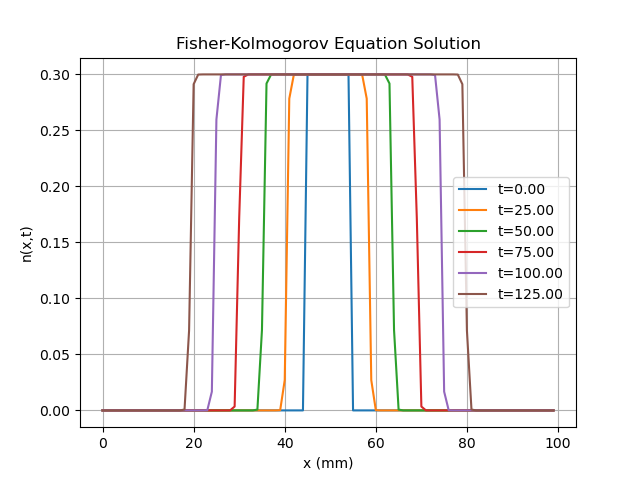
\includegraphics[width=0.5\linewidth]{FK_1D.png}
    \caption{1D Fisher-Kolmogorov Solution}
    \label{fig:enter-label}
\end{figure}\\


In two dimensions:
\[ \frac{\partial n}{\partial t} = D \left(\frac{\partial^2 n}{\partial x^2}+\frac{\partial^2 n}{\partial y^2}\right) + kn\left(1 - \frac{n}{n_{sat}}\right) \]
Parameters: $D = 0.0008 $mm$^2$/h, $k = 1$, $n_{sat} = 0.3$mm$^{-2}$, $dt = 0.01$, shown at time 10h; \hyperlink{FK_2D_Code}{Code}
\begin{figure}[h]
    \centering
    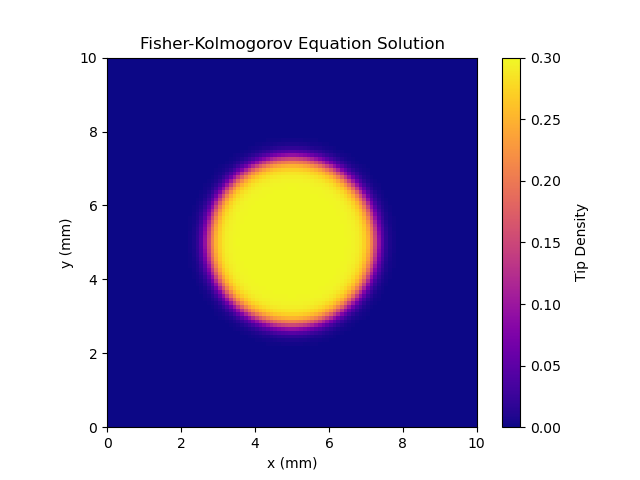
\includegraphics[width=0.5\linewidth]{FK_2D.png}
    \caption{2D Fisher-Kolmogorov Solution}
    \label{fig:enter-label}
\end{figure}


\subsection{Continuum Mean Field Model}
If we assume hyphal filament fills the space it's in completely (continuum) and we approximate the stochastic behavior of all interactions with the average (mean) behavior, we can approximate the density of hyphal filament with a continuum mean field model. 

If the length of filament deposited in one dimension by a tip growing at velocity $v$ between $t$ and $t + \Delta t$ is $v\Delta t$, and the number of tips in an area of size $(v\Delta t)^d$ is $N = n(v\Delta t)^d$,
the change in hyphal density is
\[ \Delta \rho = \frac{Nv\Delta t}{(v\Delta t)^d}\]
and the change in hyphal density, with respect to time is
\[ \lim_{\Delta t \rightarrow 0} \frac{\Delta\rho}{\Delta t} = \frac{Nv}{(v\Delta t)^d} = \frac{n(v\Delta t)^d v}{(v\Delta t)^d} = vn \longrightarrow \frac{\partial \rho}{\partial t} = vn \]
Parameters: $D = 0.0008 $mm$^2$/h, $k = 0.9$, $n_{sat} = 0.3$mm$^{-2}$, $v =240 \mu$m/h, $dt = 0.01$, shown at time 10h; \hyperlink{fk_2d_withFilament}{Code}
\begin{figure}[h]
    \centering
    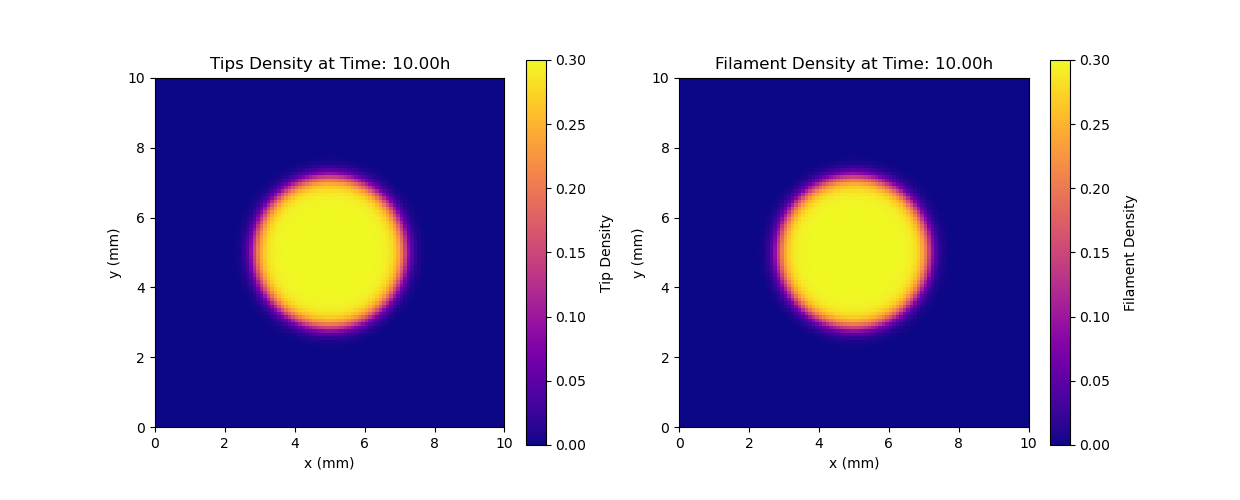
\includegraphics[width=0.9\linewidth]{FK_2D_wFilament.png}
    \caption{2D Fisher-Kolmogorov Solution for Tips and 2D Continuum Mean Field Model of Filament}
    \label{fig:enter-label}
\end{figure}

\subsection{Incorporating Processes}
\textbf{Branching: } Let the branching (tip creation events, per unit time per unit volume), with branching rate per hour $\alpha$, be modeled by \[b(n,\rho) = b(n) = \alpha n\]

Why is the branching rate not dependent on $\rho$? New tips always emerge near a growing tip \cite{Oyarte2025travelling}, so it is not directly dependent on filament density.

\textbf{Anastomosis: } The probability of an individual tip to anastomose during a time frame $dt$ is $p_f v \rho dt$. For the tips of an area of tip density $n$, this probability becomes is $p_f v \rho n dt$. Let the anastomosis rate parameter be $\beta \equiv p_f v$. The rate of anastomosis (tip annihilation events, per unit time per unit volume) can then be modeled by \[ a(n,\rho) = v p_f n \rho = \beta n \rho \] 

If we take the Fisher Kolmogorov model from earlier and replace the logistic growth term with the effects of branching and anastomosis, the tip density changes in time as follows:
\begin{align*}
    \frac{\partial n}{\partial t} &= \underbrace{b(n,\rho)}_{\text{branching}} - \underbrace{a(n,\rho)}_{\text{anastomosis}} -\underbrace{\nabla \cdot \mathbf{J}(n)}_{\text{tip movement}} \\
    &= \underbrace{\alpha n}_{\text{branching}} - \underbrace{\beta n \rho}_{\text{anastomosis}} -\underbrace{\nabla \cdot ( n\vec{v} -D\nabla n)}_{\text{tip movement}}
\end{align*}
We will keep the hyphal filament density as a continuum mean-field model:
\[ \frac{\partial\rho}{\partial t} = vn \]

As an effect, the filament saturation density found by plugging in the filament density equation into the the tip density equation and solving for steady states is  $\rho_{sat} = 2\alpha/\beta$.
Also, although we ``removed" the logistic growth term, the branching and anastomosis terms form their own logistic growth term:
\begin{align*}
    b(n, \rho) - a(n, \rho) & = \alpha n - \beta n \rho  = n(\alpha - \beta \rho) \\
    & = n(\alpha - 2\frac{\alpha\rho}{\rho_{sat}}) \text{\ \ (using $\beta = 2\alpha/\rho_{sat}$)}\\
    & = \alpha n(1 - 2\frac{\rho}{\rho_{sat}})
\end{align*}
I simulated the following model in radial coordinates with parameters $\alpha = 0.039$ tip annihilations per time per area, $beta = 0.022$ tip creations per time per area, $c = .280$ mm/h, $D = 0.0008$ mm$^2$/h, $v = .240$ mm/h, $n_{sat} = .3$mm$^{-2}$, $dt = 0.01$; $r$ is in mm and the color indicades density. \hyperlink{BA}{Code}
\begin{align*}
    \frac{\partial n}{\partial t}
    &= \underbrace{\alpha n}_{\text{branching}} - \underbrace{\beta n \rho}_{\text{anastomosis}} -\underbrace{\nabla \cdot ( n\vec{v} -D\nabla n)}_{\text{tip movement}} \\
    \frac{\partial\rho}{\partial t} &= vn
\end{align*}
\begin{figure}[h]
    \centering
    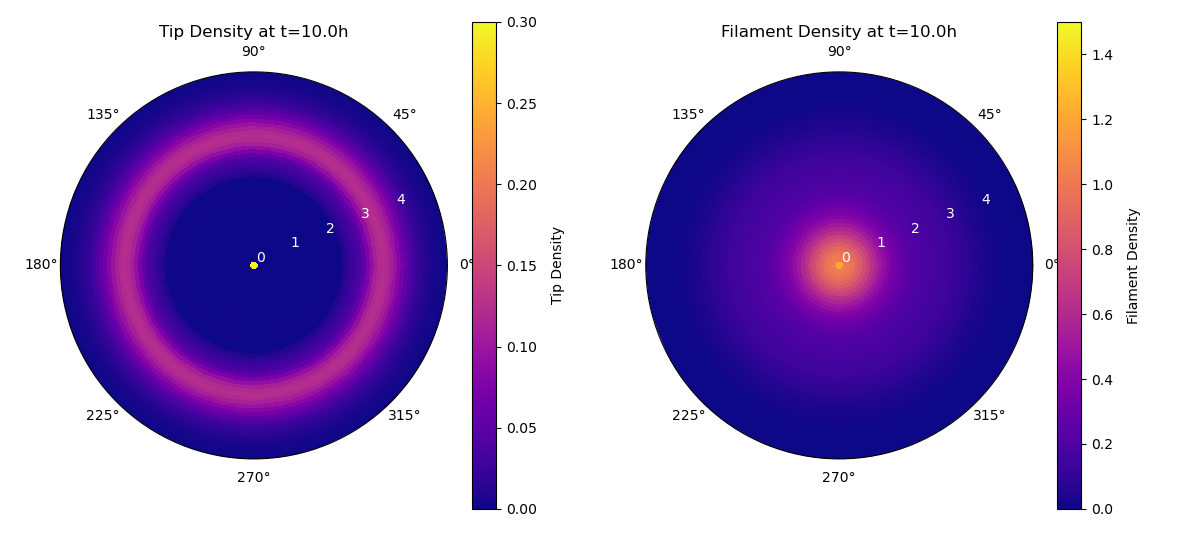
\includegraphics[width=0.9\linewidth]{withBandA.png}
    \caption{Tip and Filament Density, with Branching and Anastomosis}
    \label{fig:enter-label}
\end{figure}\\

\cite{Oyarte2025travelling} looked for asymptotically time-invariant solutions (because they measured density along a radial axis).  
In transforming $n(r,t)$ to $n(r')$ and $\rho(r,t)$ to $\rho(r')$, the model changes to 
\begin{align*}
    -c\frac{\partial\rho}{\partial r'} & = vn \\
    -c\frac{\partial n}{\partial r'} & = -b(n,\rho) - a(n,\rho) - \nabla\cdot\mathbf{J}(n) 
\end{align*}
where $c$ is velocity of wavefront in micrometers per hour.

The solutions for this model are traveling wave solutions (just as before with the Fisher Kolmogorov model). Since all effects here are dependent only on the processes on the wave-front, the solutions are pulled waves as well. This is justified mathematically by the exponential growth near zero density and approach to a (finite) saturation density.

\subsection{Brief Comments on Models}
There is a big difference in tip density results from the Fisher Kolmogorov model compared to the model with branching and anastomosis. As these shapes align with the results in \cite{Oyarte2025travelling}, I think the difference is inherent to the model. Therefore, I believe the expanding ring from the model with branching and anastomosis is probably more accurate. This could be verified directly by using data from \cite{Oyarte2025travelling}, but the data has been to large to download for me so far. Some dubious (yet to be improved) aspects of my simulations techniques are that I use a forward Euler method, and am not sure about the correctness of how I take the gradient of the flux in the model with branching and anastomosis. I also use parameters like $D$ across a variety of dimensions, assuming a 1 mm height, width, etc to be considered each time I change the dimension.

There are various alternative approaches to modeling hyphal growth, such as organelle based models \cite{King2015framework}, and biomechanical models \cite{GORIELY2003211}, and discrete grid-based models \cite{Boswell2006Development}. The traveling wave model from \cite{Oyarte2025travelling} makes sense given the data collected, which is conducive to deriving parameters like average velocity of tips, probability of anastomosis, etc, and seems to match their data as well. If I continue to work on this I am interested in models of the nutrient flows within mycelia, as well as between mycelia and plant roots. I am also curious about comparing accuracies of different modeling frameworks, and what practical applications models of hyphal networks could have. 

\bibliographystyle{plain} % We choose the "plain" reference style
\bibliography{refs} % Entries are in the refs.bib file

\section{Appendix: Code}
I wrote my code with variable names that matched the more general statements of Fisher Kolmogorov models I found, so n is used for other things like counting and u represents the tip density here, but I haven't refactored it yet. It is confusing so I've hidden the code in an appendix here, and hopefully my comments are clear enough about meanings of each variable name. Code listings should be functional individually, provided the following library dependencies are imported.
\begin{lstlisting}[language=Python, caption=Library Dependencies]
# data managemement
import numpy as np 
import pandas as pd 

# plotting
import matplotlib as mpl 
import matplotlib.pyplot as plt 
from matplotlib.axis import Axis 
import imageio
import os

# math methods
from scipy.integrate import solve_ivp 
from scipy.ndimage import convolve
\end{lstlisting}

\hypertarget{FK_1D_Code}{}
\begin{lstlisting}[language=Python, caption=1D Fisher Kolmogorov Code]
# 1-D Fisher Kolmogorov 
def fk_1d(t, u, D, r, K):
    N = len(u)
    u_t = np.zeros(N) # du/dt, initialized to 0s

    for i in range(0, N):
        # using the (second order) central difference approximation, with h=1
        # \[ f``(x) ~ \frac{f(x+h) - 2f(x) + f(x-h)}{h^2} \] 
        if (i == N - 1):
            u_xx = - 2*u[i] + u[i-1]
        elif (i == 0):
            u_xx = u[i+1] - 2*u[i]
        else:
            u_xx = u[i+1] - 2*u[i] + u[i-1]

        u_t[i] = (D * u_xx) + (r * u[i] * (1 - (u[i]/K)))
    return u_t


# Simulate 1D Fisher Kolmorogov Model
def fk_sim_1d():
    # Define parameters
    D = 0.0008      # Diffusion constant
    r = 1           # Growth rate
    K = 0.3         # tip saturation density
    T = 150         # Number of time points to evaulate at
    N = 100         # Number of points

    # Initialize vector of tip densities at each position
    u0 = np.zeros(N)
    u0[int(N/2 - 5):int(N/2 + 5)] = K
    
    # Time vector
    t_span = (0, T)
    t_eval = range(0,T,25)

    # Solve the equation using solve_ivp
    sol = solve_ivp(fk_1d, t_span, u0, args=(D, r, K), dense_output=True, t_eval=t_eval, method='RK45')

    x = range(0,N)
    plt.xlabel('x (mm)')
    plt.ylabel('n(x,t)')
    plt.title('Fisher-Kolmogorov Equation Solution')

    # Plot the solution
    for i in range(len(sol.t)):
        plt.plot(x, sol.sol(sol.t[i]), label=f't={sol.t[i]:.2f}')
    
    plt.legend()
    plt.grid(True) # add grid lines
    plt.show()

fk_sim_1d()
\end{lstlisting}

\hypertarget{FK_2D_Code}{}
\begin{lstlisting}[language=Python, caption=2D Fisher Kolmogorov Code]
# 2-D Fisher Kolmogorov using my direct interpretation of the laplacian formula
def fk_2d(u, dt, D, r, K):
    nx = len(u)
    ny = len(u[0])
    u_t = np.zeros((nx, ny))
    u_new = u

    # using the (second order) central difference approximation
    for i in range(0,nx):
        for j in range(0,ny):
            # find u_xx 
            if (i == nx - 1):
                u_xx = - 2*u[i][j] + u[i-1][j]
            elif (i == 0):
                u_xx = u[i+1][j] - 2*u[i][j]
            else:
                u_xx = u[i+1][j] - 2*u[i][j] + u[i-1][j]

            # find u_yy
            if (j == ny - 1):
                u_yy = - 2*u[i][j] + u[i][j-1]
            elif (j == 0):
                u_yy = u[i][j+1] - 2*u[i][j]
            else:
                u_yy = u[i][j+1] - 2*u[i][j] + u[i][j-1]

            u_t[i][j] = (D * (u_xx + u_yy)) + (r * u[i][j] * (1 - (u[i][j]/K)))
            u_new[i][j] = u[i][j] + dt*u_t[i][j]
    
    return u_new

# 2-D Fisher Kolmogorov using a Laplacian Kernel to approximate the second derivative
def fk_2d_conv(u, dt, dx, dy, D, r, K):
    u_new = u.copy()

    # using the Laplacian kernel approximation
    laplacian_kernel = np.array([[0,  1,  0],
                                 [1, -4,  1],
                                 [0,  1,  0]])
    u_lap = convolve(u, laplacian_kernel, mode='constant') / dx**2
    
    u_t = D * u_lap + r * u * (1 - u/K)
    u_new = u + dt*u_t
    return u_new

# Simulate Fisher Kolmorogov Model
def fk_sim_2d():
    # define parameters
    D = 0.0008      # Diffusion constant
    r = 1           # Growth rate
    K = 0.3         # tip saturation density
    
    T = 10          # Total duration
    dt = .01        # Time step
    nt = int(T/dt)  # Number of time points to evaulate at
    
    xmax = 10           # Max y value (min=0)
    ymax = 10           # Max y value (min=0)
    dx = 0.1            # Spatial step length in x
    dy = 0.1            # Spatial step length in y
    nx = int(xmax/dx)   # Number of points in x
    ny = int(ymax/dy)   # Number of points in y

    # Vector of tip densities at each position
    u = np.zeros((nx,ny))
    # Initialize to small gaussian at center
    x, y = np.linspace(0, xmax, nx), np.linspace(0, ymax, ny)
    X, Y = np.meshgrid(x, y, indexing='ij')
    x0, y0 = int(xmax/2), int(ymax/2)
    sigma_u = 0.5 
    u = K*np.exp(-((X-x0)**2 + (Y-y0)**2) / (2 * sigma_u**2))
    
    # Set up plot
    plt.ion()
    fig, ax = plt.subplots()
    im = ax.imshow(u, extent=[0, xmax, 0, ymax], vmin=0, vmax=K, 
                    origin='lower', cmap='plasma')
    fig.colorbar(im)
 
    # Plot at each time step
    for n in range(nt):
        # comment out either line to choose which method to use to update u
        # u = fk_2d(u, dt, D, r, K) # direct implementation of Laplacian formula
        u = fk_2d_conv(u, dt, dx, dy, D, r, K) # Convolution of Laplacian kernel
    
        if n % 10 == 0:
            im.set_data(u)
            ax.set_title(f'Time: {n*dt:.2f}')
            fig.canvas.draw_idle()
            plt.pause(0.01)

    # additional plot settings
    plt.ioff()
    plt.xlabel('x (mm)')
    plt.ylabel('y (mm)')
    plt.title('Fisher-Kolmogorov Equation Solution')
    plt.show()

fk_sim_2d()
\end{lstlisting}

\hypertarget{fk_2d_withFilament}{}
\begin{lstlisting}[language=Python, caption=2D Fisher Kolmogorov (Tips) with Continuum Mean Field Model (Filament) Code]
# 2D Fisher Kolmogorov Model of Tip Density
# and 2D Continuum Mean Field Model of Filament Density
def fk_2d_withFilament():
    # units milimeters
    r = 0.9         # growth rate
    alpha = 0.039   # branching rate
    beta = 0.022    # anastomosis rate 
    c = .280        # speed of traveling wavefront
    D = 0.0008      # diffusion constant 
    v = .240        # velocity of tips
    K = .3          # tip saturation density
    
    T = 10          # Total duration
    dt = .01        # Time step
    nt = int(T/dt)  # Number of time points to evaulate at
    
    xmax = 10           # Max y value (min=0)
    ymax = 10           # Max y value (min=0)
    dx = 0.1            # Spatial step length in x
    dy = 0.1            # Spatial step length in y
    nx = int(xmax/dx)   # Number of points in x
    ny = int(ymax/dy)   # Number of points in y

    # intialize u and rho
    x, y = np.linspace(0, xmax, nx), np.linspace(0, ymax, ny)
    X, Y = np.meshgrid(x, y, indexing='ij')
    x0, y0 = 5, 5
    sigma_u = 0.5 
    # tip density - starting with a small gaussian
    u = K*np.exp(-((X-x0)**2 + (Y-y0)**2) / (2 * sigma_u**2))
    # filament density - starting with 0
    rho = np.zeros((nx,ny))

    # set up plots
    plt.ion()
    fig, ax = plt.subplots(nrows=1, ncols=2, figsize=(10,5))
    ax[0].grid(False)
    ax[1].grid(False)
    imu = ax[0].imshow(u, extent=[0, xmax, 0, ymax], vmin=0, vmax=K, origin='lower', cmap='plasma')
    imrho = ax[1].imshow(u, extent=[0, xmax, 0, ymax], vmin=0, vmax=K, origin='lower', cmap='plasma')
    fig.colorbar(imu).set_label('Tip Density', labelpad=10)
    fig.colorbar(imrho).set_label('Filament Density', labelpad=10)
    ax[0].set_xlabel('x (mm)')
    ax[1].set_xlabel('x (mm)')
    ax[0].set_ylabel('y (mm)')
    ax[1].set_ylabel('y (mm)')
 
    # plot at each time step
    for n in range(nt+1):
        rho_t = v*u
        laplacian_kernel = np.array([[0,  1,  0],
                                 [1, -4,  1],
                                 [0,  1,  0]])
        u_lap = convolve(u, laplacian_kernel, mode='constant') / dx**2
        u_t = D * u_lap + r * u * (1 - u/K)

        u = u + dt*u_t
        rho = rho + dt*rho_t
        
        if n % 10 == 0: # plot at time step (every 10 steps)
            imu.set_data(u)
            imrho.set_data(u)
            ax[0].set_title(f'Tips Density at Time: {n*dt:.2f}h')
            ax[1].set_title(f'Filament Density at Time: {n*dt:.2f}h')
            fig.canvas.draw_idle()
            plt.pause(0.01)

    # plot
    plt.ioff()
    plt.show()

fk_2d_withFilament()
\end{lstlisting}

\hypertarget{BA}{}
\begin{lstlisting}[language=Python, caption=Tip and Filament Density (with Branching and Anastomosis) Code]
# units milimeters
alpha = 0.039   # branching rate
beta = 0.022    # anastomosis rate 
c = .280        # speed of traveling wavefront
D = 0.0008      # diffusion constant 
v = .240        # velocity of tips
K = .3          # tip saturation density

T = 10          # Total duration
dt = .01        # Time step
nt = int(T/dt)  # Number of time points to evaulate at

rmax = 5           # Max r value
dr = 0.1            # Spatial step length in r
nr = int(rmax/dr)   # Number of points in r
ntheta = 100        # Number of points in theta
dtheta = 2 * np.pi / ntheta # Spatial step length in theta

r, theta = np.linspace(0,rmax, nr), np.linspace(0,2*np.pi,ntheta)
R, THETA = np.meshgrid(r,theta, indexing='ij')

u = np.zeros((nr,ntheta))
rho = np.zeros((nr,ntheta))

u[:, :] = np.exp(-R**2)  # smooth Gaussian seed
rho[:, :] = np.exp(-R**2)

# set up plot
plt.ioff()
figs, axes = plt.subplots(nrows=1, ncols=2, figsize=(10,5), subplot_kw={'projection': 'polar'})
axes[0].grid(False)
axes[1].grid(False)
axes[0].tick_params(axis='y', colors='white') 
axes[1].tick_params(axis='y', colors='white') 

imu = axes[0].pcolormesh(THETA, R, u, cmap='plasma',  vmin=0, vmax=K)
imrho = axes[1].pcolormesh(THETA, R, rho, cmap='plasma',  vmin=0, vmax=1.5)
figs.colorbar(imu).set_label('Tip Density', labelpad=10)
figs.colorbar(imrho).set_label('Filament Density', labelpad=10)

plt.tight_layout()


# plot at each time step
for n in range(nt+1):
    R_nonzero = R + 1e-8  # to avoid divide-by-zero

    u_r = np.gradient(u, dr, axis=0)
    u_theta = np.gradient(u, dtheta, axis=1)
    J = v * u - D * u_r

    div_r = (1 / R_nonzero) * np.gradient(R*J, dr, axis=0)
    div_theta = (1 / R_nonzero**2) * np.gradient(D * u_theta, dtheta, axis=1)
    divergence = div_r + div_theta

    u_t = (alpha*u) - (beta*u*rho) - divergence
    rho_t = v*u

    u = u + u_t*dt
    rho = rho + rho_t*dt
    u = np.clip(u, 0, K)


    if n % 10 == 0: # plot every 10 time steps

        axes[0].collections.clear()
        axes[1].collections.clear()
        
        axes[0].pcolormesh(THETA, R, u, shading='auto', cmap='plasma', vmin=0, vmax=K)
        axes[1].pcolormesh(THETA, R, rho, shading='auto', cmap='plasma', vmin=0, vmax=1.5)
        
        axes[0].set_title(f'Tip Density at t={n*dt:.1f}h')
        axes[1].set_title(f'Filament Density at t={n*dt:.1f}h')

        figs.canvas.draw_idle()
        plt.pause(0.01)

plt.ioff()
plt.show()
\end{lstlisting}

\end{document}



